%--------------------------------------------------------------------------- 
% Chapter 2 - Related technologies %

%--------------------------------------------------------------------------- 
\section{Related technologies} 
%---------------------------------------------------------------------------

\subsection{K-WfGrid facilities}

\label{ssec:kwfgrid}

K-WfGrid, which stands for Knowledge-based Workflow System for Grid Applications (\cite{KWfGrid1, flow-cgw04, wct-kwf-book-07}), is both middleware solution that aims in setting up infrastructure for the future Grid environments and consortium of institutions participating in development of this solution. To solve problems caused by dynamic and complex nature of Grid environments, the consortium adopts approaches envisioned by Semantic Web, agent technologies and Grid communities. As an outcome, K-Wf Grid system assists users in the creation of Grid workflows using rule-based expert system. The system adopts ontological descriptions of the environment and applications.

The implemented system, is capable of handling the whole life cycle of workflow, which includes:

\begin{itemize}

\item{semi-automatic composition of application workflow} \item{execution of composed workflow} \item{monitoring performance of execution} \item{analyzing monitoring results} \item{capturing the knowledge contained in this information and tries to {\bf reuse} it in order to construct more efficient, future workflows} \end{itemize}

The main workflow composition functionality is defined as a transformation of a user request document into a solution workflow document in the same data format. The input document must be written using fixed notation - \emph{GWorkflowDL} and may contain some parts of workflow already specified. Parts that are still undefined (called \emph{Unsatisfied Dependency}) contain specification of data that are required at a certain stage of processing. System must find suitable providers of those data in order to generate the whole workflow. Providers, in the form of one or more Grid services are looked up in ontological registry. The workflow is considered to be done, when all unsatisfied dependencies are resolved.

%---------------------------------------------------------------------------

\subsection{OMIS}

\label{ssec:omis}

OMIS, On-Line Monitoring Interface Specification, is another example of efforts aiming at standardization and interoperability between grid monitoring tools. Work on this project was started in 1995. As an outcome, an interface specification in three versions was created: OMIS 1.0~\cite{OMIS1}, 2.0~\cite{OMIS2} and 2.1.

The main purpose of this project is to define an interface that will allow communication between development tools (e.g. debuggers, performance analyzers or load balancers) and parallel programs running in distributed environment. The researchers had three main goals to achieve: to define an interface that will be extensive and complete to allow usage in existing tools, to allow extendibility and usage in tools not known yet and finally to allow high adaptability to current and future programming paradigms (shared memory, remote procedure call or client/server).

Authors introduced two sub-interfaces to achieve those goals. The first one is for communication between tool and program (monitor/program-interface). The second one lies between tool and monitors (tool/monitor-interface) and has additional extension points. The illustration of this model can be found in Figure~\ref{fig:omis}.

\begin{figure}[ht]

\centering

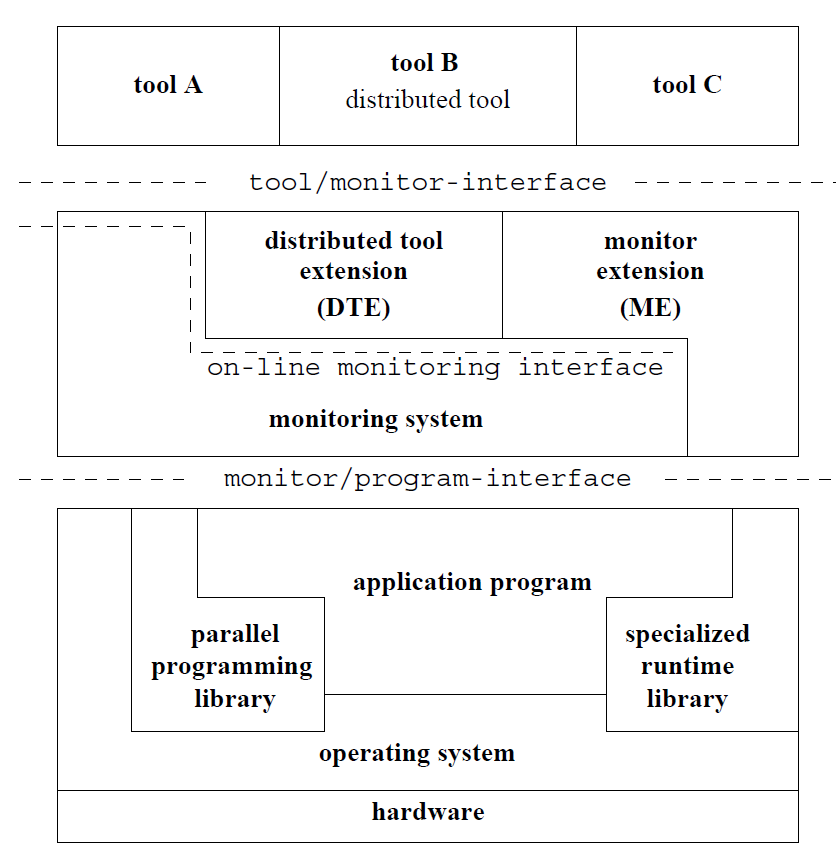
\includegraphics[width=0.6\textwidth]{omis} \caption{OMIS System Model} \label{fig:omis}

\end{figure}

The OMIS standard defines two kinds of monitoring request - unconditional and conditional ones. Unconditional services specify a set of actions to be performed immediately. It can be interpreted as querying a monitoring mode, where results are obtained instantly and unconditionally. Requests of this type are composed just of one and more information or manipulation services. It creates a request/response communication model. In the second mode, requests contain an event service and a set of actions. In this mode, request tells the monitoring system to execute actions substantially. It creates a publish/subscribe communication model.

\subsection{GMA}

\label{ssec:gma}

GMA stands for Grid Monitoring Architecture~\cite{GMA1,GMA2}. It was originally introduced by Global Grid Forum in 2002. A need to create a shared interface for monitoring grid resources emerged, when several groups of researchers started working on systems facilitating grid monitoring and decided that those tools should be interoperable. The standard is composed of three, high level, types of components. Figure~\ref{fig:gma} depicts them and their relationships.

\begin{figure}[ht]

\centering

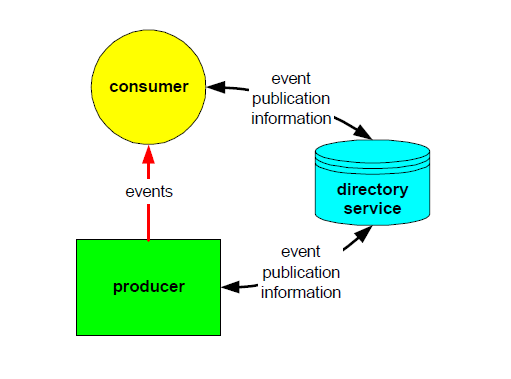
\includegraphics[width=0.6\textwidth]{gma} \caption{GMA Components} \label{fig:gma}

\end{figure}

GMA-compatible systems should operate on data that are time stamped performance events. Those events are typed collections of structured data. Measurement data flow always in one direction - from a producer to consumer. Additionally, directory service acts as mediator between them and its work is finished directly after successful establishment of communication link. GMA supports two data exchange models - publish/subscribe (similar to CORBA Event Service) and query/response. What is worth noting, communication may be initiated by both component types - either by a producer or a subscriber.